\documentclass[11pt]{article}
\usepackage[utf8]{inputenc}
\usepackage{graphicx}
\usepackage[spanish]{babel}
\title{\textbf{Práctica 2}}
\author{Javier Sáez, Laura Garrido, Daniel Pozo, Luis Ortega}
\date{}
\begin{document}

\maketitle
\section{Newton}
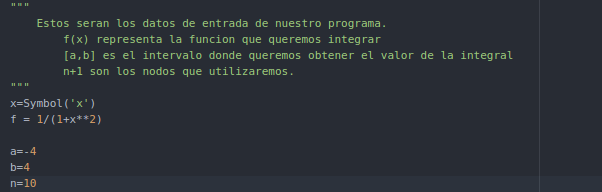
\includegraphics[scale=0.6]{n1}
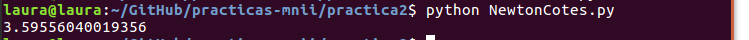
\includegraphics[scale=0.6]{n2}

\section{Simpson}
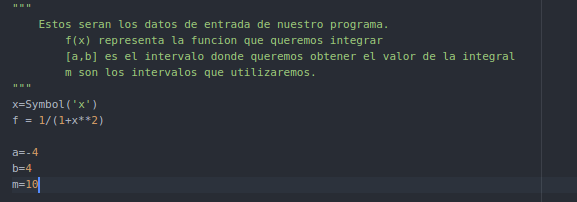
\includegraphics[scale=0.6]{s1}
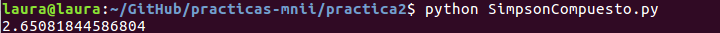
\includegraphics[scale=0.6]{s2}

\section{Romberg}
En este caso, lo que se intenta es aproximar la integral de la función $log(x)$ en el intervalo $[1,2]$ con $n=10$ nodos.
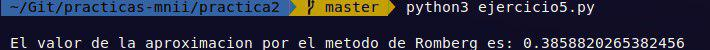
\includegraphics[scale=0.6]{r1}






\end{document}
